\label{sec:piezo_theor}
В материалах обладающих пьезоэлектрическими свойствами существует
линейная связь между механическим напряжением и электрической поляризаций
(прямой пьезоэлектрический эффект) или между механической деформацией
и приложенным электрическим полем (обратный пьезоэлектрический эффект).

\begin{figure}[H]
  \centering
  \subfloat[Деформация кристаллической структуры вызывает появление
  разности электрических потенциалов на гранях кристалла (прямой пьезоэлектрический эффект)
  ]{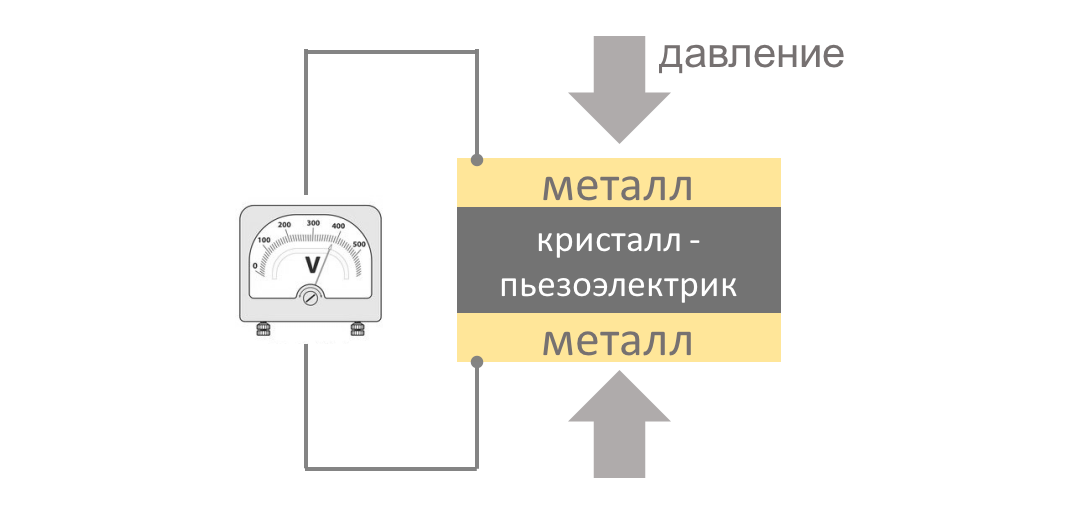
\includegraphics[width=0.4\textwidth]{images/piezo_ther_1.png}}
  \hfill
  \subfloat[Внешнее электрическое поле вызывает деформацию кристалла
  (обратный пьезоэлектрический эффект)]{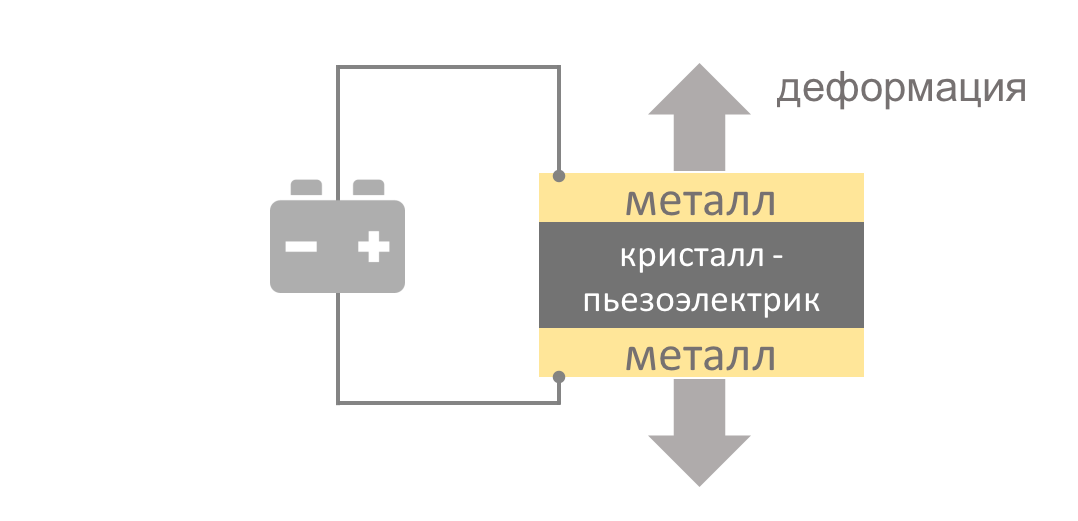
\includegraphics[width=0.45\textwidth]{images/piezo_ther_2.png}}
  \caption{Свойство пьезоэлектрического кристалла в его простейшем виде}
  \label{ris:piezo_is}
\end{figure}

Согласно определению обратного пьезоэлектрического эффекта,
приложенное внешнее электрическое поле $\vec{E}$ является причиной возникновения
в кристаллическом материале деформаций $r_i$. Вектор деформаций пропорционален
величине приложенного напряжения и зависит от пьезоэлектрических свойств материала
в данном направлении $d$. Модуль пьезоэлектрических деформаций $d$ является
матричной 3х6 \cite{kedi_1949,Newnham_2005}.


\begin{equation}
  r_j = d_{ij}E_i
  \label{eq:piezomodule}
\end{equation}
где $i = (1,2,3) = (x,y,z)$, $j = (1,2,3,4,5,6)$, $E_i$ - компонента напряженности электрического поля.

Исходя из уравнения (\ref{eq:piezomodule}) можно судить о том, что поле приложенное в каком-либо из
направлений может вызывать деформацию кристалла в любом направлении с коэффициентом пропорциональности $d_{ij}$.

Компоненты деформации  $r_1$, $r_2$ ...$r_6$ можно также обозначать  через $x_x$, $y_y$, $z_z$,
$y_z$, $z_x$ и $x_y$ (обозначения Кирхгофа)  \cite{kedi_1949}.

Они связаны со смещением следующим образом:
\begin{figure}[H]
  \centering
  \subfloat[]{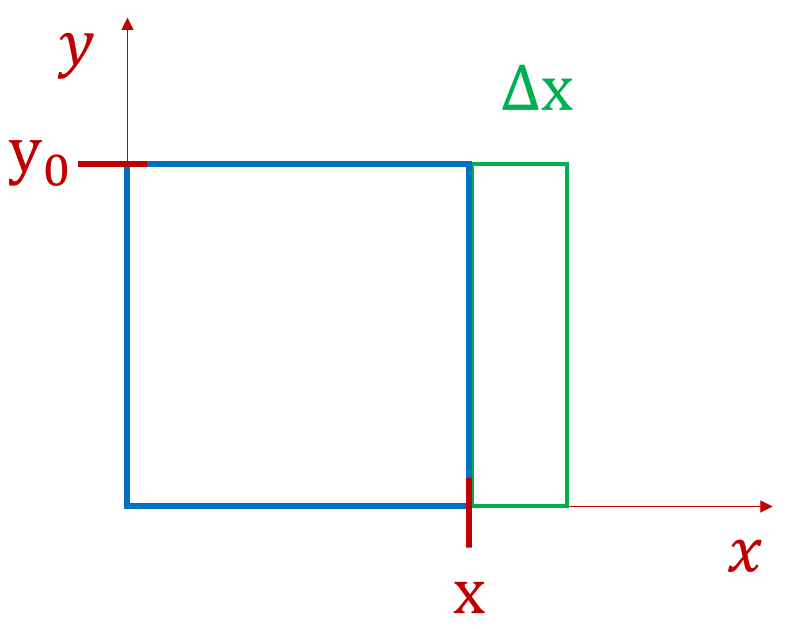
\includegraphics[width=0.45\textwidth]{images/x_x_2d.png}}
  \hfill
  \subfloat[]{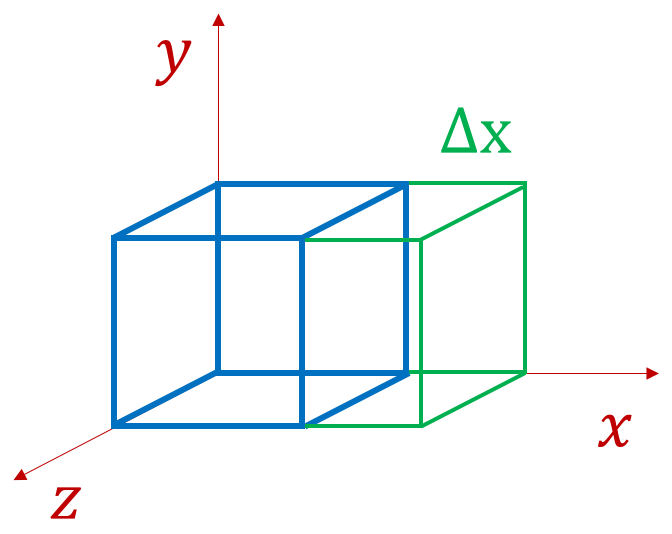
\includegraphics[width=0.45\textwidth]{images/x_x_3d.png}}
  \caption{К объяснению деформации растяжения и сжатия. $r_1= x_x = \frac{\Delta x}{x_0} $}
  \label{ris:}
\end{figure}

\begin{figure}[H]
  \centering
  \subfloat[на плоскости]{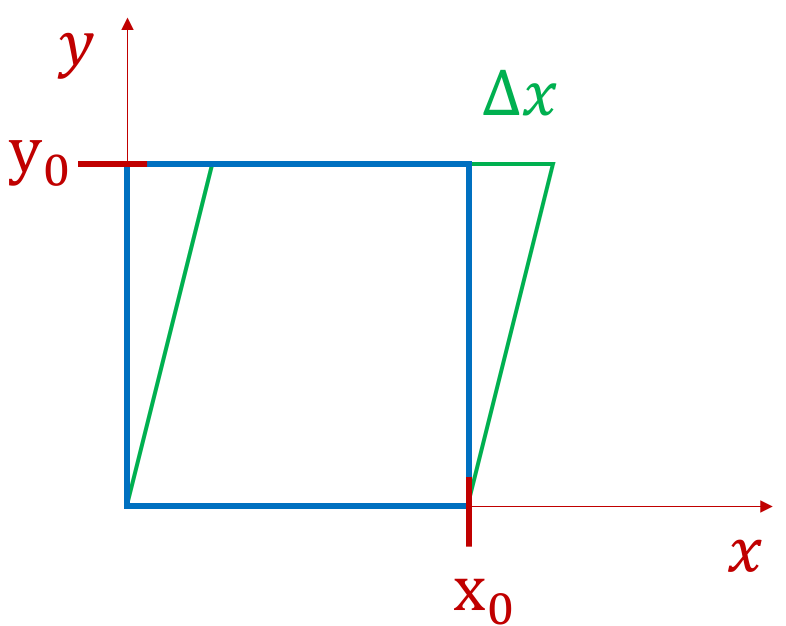
\includegraphics[width=0.45\textwidth]{images/x_y_2d.png}}
  \hfill
  \subfloat[в объеме]{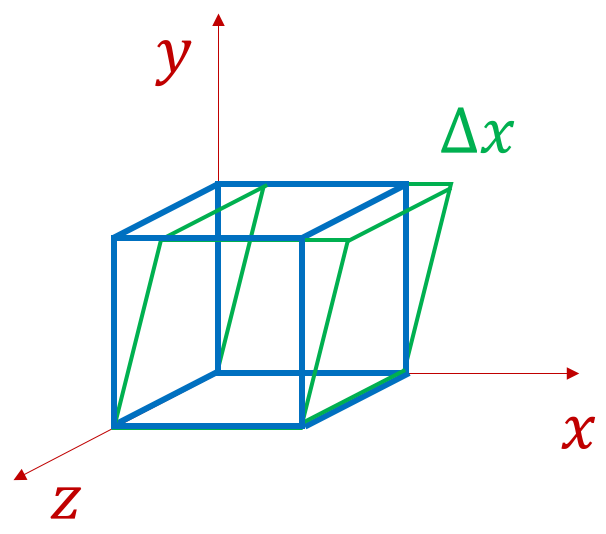
\includegraphics[width=0.45\textwidth]{images/x_y_3d.png}}
  \caption{К объяснению деформации сдвига. $r_6= x_y = \frac{\Delta x}{y_0} $}
  \label{ris:x_y_2d}
\end{figure}

Поясняя рисунок \ref{ris:x_y_2d}, в случае деформации сдвига обозначают
компоненты векторов в плоскости которых происходит деформация. Если $x_y$ и $y_x$
налагаются одновременно, такую деформацию можно представить в виде одного из
смещений с учетом поворота всего образца, так если например $x_y = y_x$, произойдет
просто удвоение одной из компонент (рисунок \ref{ris:2x_y_1}). С математической
точки зрения отождествление компонент $x_y$ с $y_x$ уменьшает число компонент
общего тенора деформаций.

\begin{figure}[H]
  \centering
  \subfloat[на плоскости]{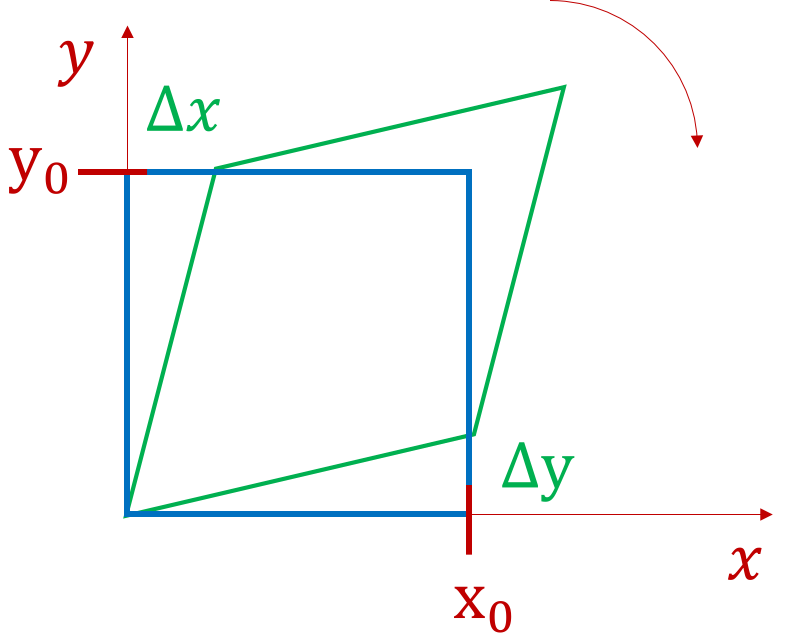
\includegraphics[width=0.45\textwidth]{images/2x_y_1.png}}
  \hfill
  \subfloat[в объеме]{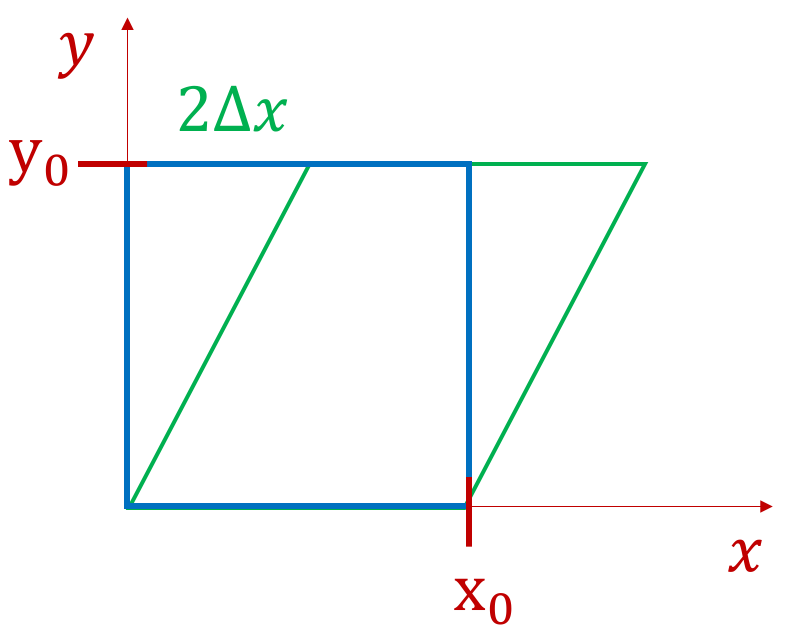
\includegraphics[width=0.45\textwidth]{images/2x_y_2.png}}
  \caption{Отождествление компонент деформации $x_y$ с $y_x$ }
  \label{ris:2x_y_1}
\end{figure}

В развернутой форме выражение (\ref{eq:piezomodule}) выглядит как

\begin{equation}
  \begin{pmatrix}
  r_1 \\
  r_2 \\
  r_3 \\
  r_4 \\
  r_5 \\
  r_6
  \end{pmatrix}
   = \begin{pmatrix}
  d_{11} & d_{21}  & d_{31} \\
  d_{12} & d_{22}  & d_{32} \\
  d_{13} & d_{23}  & d_{33} \\
  d_{14} & d_{24}  & d_{34} \\
  d_{15} & d_{25}  & d_{35} \\
  d_{16} & d_{26}  & d_{36}
  \end{pmatrix}
  \begin{pmatrix}
  E_1 \\
  E_2 \\
  E_3
  \end{pmatrix}
  \label{eq:piezomodule_matrica}
\end{equation}

В общем случае все 18 пьезомодулей не зависимы друг от друга. Однако
под действием операции симметрии кристалл должен должен полностью совместиться с
самим собой и это касается не только его строения, но и любого физического свойства.
Исходя из принципа Неймана \cite{Shaskolska_1984}, физические свойства, в частном случае
пьезоэффект, по кристаллографически эквивалентным направлениям должны быть одинаковыми.
Таким образом, пьезоэлектрический эффект может возникнуть в кристаллах, лишенных центра
симметрии. В 11 классах точеной группы симметрии из 32 нет полярных направлений,
а значит в кристаллах этих классов не может возникать пьезоэффект. Для остальных
классов, некоторые пьезомодули могут обратиться в нуль из-за наличия симметрии.
Другими словами, чем выше симметрия, тем меньше число независимых пьезомодулей.
Некоторые матрицы пьезомодулей $d$ приведены в (\ref{sec:piezo_matrix}).
